%%%%%%%%%%%%%%%%%%%%%%%%%%%%%%%%%%%%%%%%%%%%%%%%%%%%%%%%%%%%%%%%%%%%%%%%%%%%%%%
% | - Structural analysis of IrO2 and IrO3 oxides %%%%%%%%%%%%%%%%%%%%%%%%%%%%%
% %%%%%%%%%%%%%%%%%%%%%%%%%%%%%%%%%%%%%%%%%%%%%%%%%%%%%%%%%%%%%%%%%%%%%%%%%%%%%
% TODO: Synthax for calling subplots in figure Figure 1.d or Figure 1.d)
% TODO: "we note that ..." is used a few times Kirsten
%
% Important Points:
%   * A good candidate set is a set of materials that have a large degree of 'structural diversity'
%
%   * We can make an analogy between the shape of these plots and typical van-der Waals curves
%     * I would argue that the tails are much less steep than a van-der Waals curve because in most cases the there is still a large degree of bonding
%       * Essentially these systems can create more and more 'porous' structures as the density is decreases, which allows us to get really large porous structures
%         * A good point can be made here that these types of systems could be useful for battery applications
%           * Pores are good in this context I think?
%
%
%   * The main coordination environments are 6 and 4-fold coordinated (Ir-O4/6 units)
%     * This is consistent with crystal field theory, or literature, etc.
%     * 6/4-coord accounts for TEMP percent of the IrO2/3 candidate space
%       * TODO Get these numbers
%     * There are in addition to 6/4-coord, a lot of other types of coordination environments
%       * A lot of these are simply weird, aphysical structures for sure
%         * Unassociated oxygens
%           * Singly-associated (part of N-hedra)
%           * Completely un-unassociated O atoms, just randomly placed in unit cell
%
%         * Especially at the extreme ends of the average coord metric
%       * But there are also a lot of legitimate coordination environments
%         * I've manually parsed the dataset and found
%
%   * There is a lot to say about the different kinds of 100% corner sharing octahedral IrO3 systems
%     * There are a lot of these systems that differ in subtle ways
%       * Basically octahedra can be "rotated" in different directions, making them distinct
%
%   * Interesting types of systems
%     * Layered systems (A lot of variety here)
%     * Cubic coordination environments (A few cool looking examples)
%     * New coordination environments
%       * TODO Remind myself again of these
%
%   * IrO2 has more 4-fold coordinated systems than IrO3
%     * Makes sense, the more oxygens you have the more oxygen-rich motifs are favored
%   * IrO2 has large "dip" in the EvsV "convex hull" while IrO3 has a much more shallow increase in energy as you move to the right from the most stable polymorph
%     * This is probably due to the fact that IrO3 can create more porous layered structures
%
% NOTES:
%   * Describe convex hull, classes of structures (\ce{$\alpha$-AlF3} like, rutile like, and layered, should be segregated in hull plot)
%   * Describe structures within each class, cite lit where appropriate
% __| %%%%%%%%%%%%%%%%%%%%%%%%%%%%%%%%%%%%%%%%%%%%%%%%%%%%%%%%%%%%%%%%%%%%%%%%%


% ################################# Paragraph #################################
% %%%%%%%%%%%%%%%%%%%%%%%%%%%%%%%%%%%%%%%%%%%%%%%%%%%%%%%%%%%%%%%%%%%%%%%%%%%%%
% TEMP
% %%%%%%%%%%%%%%%%%%%%%%%%%%%%%%%%%%%%%%%%%%%%%%%%%%%%%%%%%%%%%%%%%%%%%%%%%%%%%
% | - Paragraph start
% There should be a paragraph which discussed the structural drift and performance/acceleration in more detail
% I would use the updated version of Figure 2c.

% ###################################################################
Here we assess the structural variety of the AL dataset consisting of 448 \IrOtwo and 258 \IrOthree unique polymorphs,
where the relation between the enthalpy of formation and the inverse atomic density (Volume/atom) is shown in Figure~\ref{fig:E_vs_V}a and b.
%
Here, a large variety in structure densities and coordination environments is desirable, since this will enable us to discover novel systems.
%
To obtain a physically meaningful cutoff for the formation enthalpy above which materials are unlikely to be synthesizabl, we computed the metastability limits for \IrOtwo and \IrOthree relative to their amorphous phases using the methodology of Persson \latin{et. al.}~\cite{Aykol2018}.
%
% \textbf{you need to explain what this means, that they were computed using a previously reported algorithm (cite Murat's paper) and point to an SI section with the values.  is not clear where in the figure this is. Raul can you add this part?}
The computed metastability limits were computed to be -0.33 and -0.34 eV/atom for \IrOtwo and \IrOthree, respectively,
and are displayed as horizontal lines in Figure~\ref{fig:E_vs_V}a and b.
%
There are XX and XX polymorphs for \IrOtwo and \IrOthree, respectively, that were found to be under the meta-stability line, and are therefore predicted to be meta-stable.
%
These values are almost identical, possibly indicating that the energy of the amourphous phases are insenstivie to the exact stoicheometry.
%
Measuring the metastability relative to the hull for each stoicheometry yields a metastability window of 0.5 and 0.3 eV/atom for \IrOtwo and \IrOthree, respectively.
% __|

% ################################# Paragraph #################################
% %%%%%%%%%%%%%%%%%%%%%%%%%%%%%%%%%%%%%%%%%%%%%%%%%%%%%%%%%%%%%%%%%%%%%%%%%%%%%
% There is a large variety in density on this plot
% IrO3 has a small dependance on the volume
% %%%%%%%%%%%%%%%%%%%%%%%%%%%%%%%%%%%%%%%%%%%%%%%%%%%%%%%%%%%%%%%%%%%%%%%%%%%%%
% | - Paragraph start
We note that for both compositions,
there is a large variety in density (from \textbf{XYZ} to \textbf{XYZ}),
such that both low volume (dense) and high volume (porous) structures are represented.
%
As expected \textbf{why do you expect this?}, the most stable systems are found at low volume, \textbf{can we change this to ``at the low end of the volume range (xyz to xyz)''}
where the shape of envelope curve (lowest energy for a given volume) is analogous to the shape of the Lennard-Jones potential. \textbf{is this important or expected?}
%
% NOTE Can make a comment about the fact that these porous species may be over-stabilized with PBE DFT
However, for \IrOthree there is a comparitively weak relationship between the energy and volume,
such that even highly porous structure are within the meta-stablity energy range.
%
We note that the stability of highly porous systems has a tendency to be overestimated on the DFT+GGA level, where van der Walls interactions should be included for a better description.
%
% COMBAK Explain this point better, this has to do with the oxidation state, coordination preservation rules that I've been playing around with
This property is likey due to the fact that \IrOthree's oxidatation state can more can form readily form layered or porous structures.
%
(We note that the stability of highly porous systems has a tendency to be overestimated on the DFT+GGA level, where van der Walls interactions should be included for a better description). \textbf{unclear what you mean here, vdw is attractive so shouldn't it just make them more stable?}
% __|


% ################################# Paragraph #################################
% %%%%%%%%%%%%%%%%%%%%%%%%%%%%%%%%%%%%%%%%%%%%%%%%%%%%%%%%%%%%%%%%%%%%%%%%%%%%%
% Explaining coordination motiff distribution (octahedral, tetrahedral
% %%%%%%%%%%%%%%%%%%%%%%%%%%%%%%%%%%%%%%%%%%%%%%%%%%%%%%%%%%%%%%%%%%%%%%%%%%%%%
% | - Paragraph start
%
The structures have been classified with respect to the Ir-O coordination environment
(such as octahedral, square pyramidal, tetrahedral, cubic, etc.),
by using the chemEnv package, developed by Waroquiers et. al. \cite{Waroquiers2017} and implemented in pymatgen \cite{Ong2013}.
%
Although the dataset was found to contain a large range of coordination environments (ranging from \textbf{xyz to xyz}),
structures with a coordination number of 6 (octahedreal) or 4 (tetrahedreal) were found to be most prevalent
(accounting for roughly TEMP percent of all structures)
and have been highlighted in blue and red respectively in Figure~\ref{fig:E_vs_V}a and b.
%
% \textbf{this is kind of vague, do you mean the most stable or most of the most stable?}
For both \IrOtwo and \IrOthree the most stable candidates are seen to have an octahedral oxygen coordination,
a common coordination motiff found in many other metal oxides.\cite{Waroquiers2017}
%
% This has to be expanded upon or else maybe dropped, we can discuss
%% \textbf{I don't understand the end of this sentence.  Give some information of how this applies to your structures.}
The arrangement of the octahedreal units, which are connected through either corner-, edgesharing,
can furthermore be used to classify the structures, that typically has a combination of the two.
% __|


% ################################# Paragraph #################################
% %%%%%%%%%%%%%%%%%%%%%%%%%%%%%%%%%%%%%%%%%%%%%%%%%%%%%%%%%%%%%%%%%%%%%%%%%%%%%
% TEMP
% %%%%%%%%%%%%%%%%%%%%%%%%%%%%%%%%%%%%%%%%%%%%%%%%%%%%%%%%%%%%%%%%%%%%%%%%%%%%%
% | - Paragraph start
In Figure~\ref{fig:E_vs_V}c and d, a selection of meta-stable structures is shown for \IrOtwo and \IrOthree respectively.
%
%\textbf{what experiments?  is this  heats of formation?}
For \IrOtwo, we found rutile to be the most stable,
in correspondence with experiment \cite{}.
%
%\textbf{experimentally?  it is not clear here if you mean just the geometries or that these materials have been reported in the expt. literature}
% TODO Make active voice
Also, we found several of the well-know \IrOtwo crystal structures, including columbite, purite, brookite and anatase (not all shown).
%
For \IrOthree the five most stable systems were shown in Figure~\ref{fig:iro2_al},
and have been labeled with numbers (1)-(5) in Figure~\ref{fig:E_vs_V} b.
%
% \textbf{why?}
However, we have identified several additional meta-stable structures, including 2D(i), highly porous(iii) and 1D(v) polymorphs with varying degrees of poursity and conectivity,
which could be interesting for battery applications \cite{}.
%
% \textbf{try not to use ``we note that", it is generally always better to motivate why you are noting that}
% \textbf{the labeling scheme jumping between two figures is a little confusing here, and it obfuscates the point I think you are trying to make in this last sentence}
We note that the \IrOthree Cmcm polymorph in Figure~\ref{fig:E_vs_V}d (iv) is the the lowest energy \IrOthree structure on Materials Project
(see Materials Project entry mp-1097041~\cite{mp-1097041}).
% __|



% | - Figure | Energy vs. Volume (motif distribution)
\begin{figure*}[!htb]
\centering
\makebox[\textwidth][c]{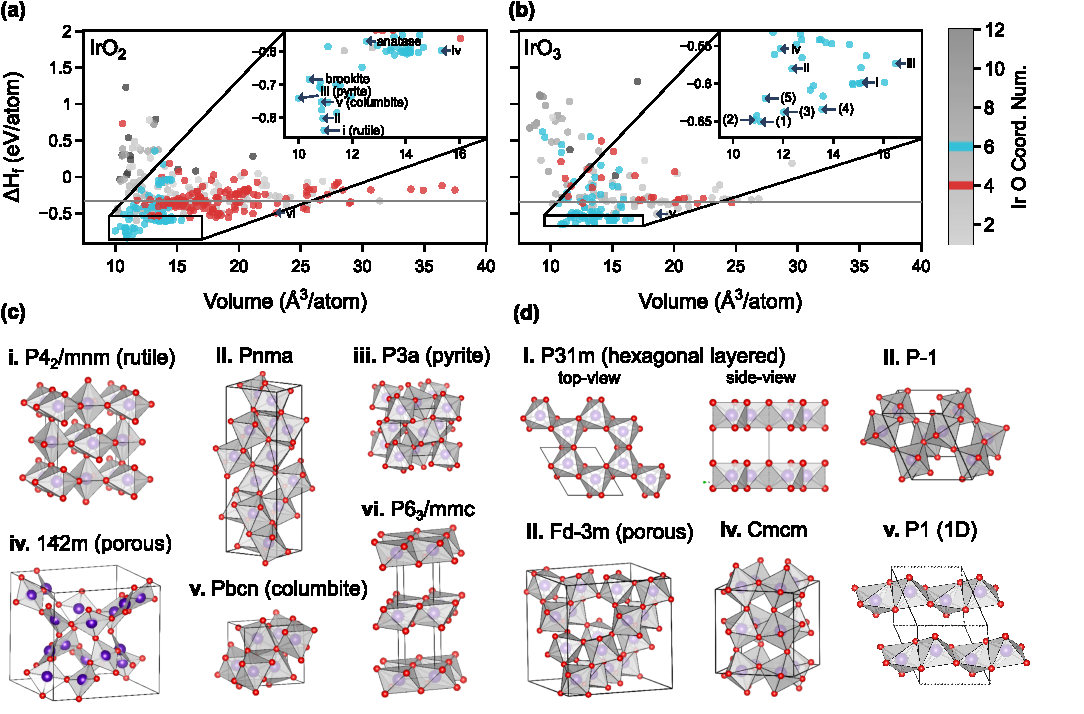
\includegraphics[
width=\textwidth,height=\textheight,keepaspectratio]
{02_figures/e_vs_v_motiffs.pdf}
}
\caption{\label{fig:E_vs_V}
%
Enthalpy of formation for the \num{448} \IrOtwo (a) and \num{258} \IrOthree (b) structures in the candidate data set plotted against the volume per atom.
%
Insets in the low energy region for (a) and (b) are shown.
%
The color bar represents the average coordination number between Ir and O, with 6 (octahedra) and 4 (tetrahedra) highlighted.
%
(c) and (d), select \IrOtwo and \IrOthree polymorph structures.
}
\end{figure*}
% __|






% | - __old__
% We classified the structures with respect to the Ir-O coordination environment (such as octahedral, square pyramidal, tetrahedral, cubic, etc.), by using the chemEnv package, developed by Waroquiers et. al. \cite{Waroquiers2017} and implemented in pymatgen \cite{Ong2013}. Although the dataset contains  coordination environments ranging from \textbf{xyz to xyz}, structures with a coordination number of 6 (octahedreal) or 4 (tetrahedreal) are the most prevalent and are highlighted in blue and red respectively in Figure \ref{fig:E_vs_V} a) and b). For both \IrOtwo and \IrOthree the most stable candidates are seen to have an octahedreal oxygen coordination\textbf{this is kind of vague, do you mean the most stable or most of the most stable?} , which is generally favored by many other metal oxides. \cite{Waroquiers2017} The arrangement of the octahedreal units, which are connected through either corner- or edge-sharing, can furthermore be used to classify the structures, that typically has a combination of the two. \textbf{I don't understand the end of this sentence.  Give some information of how this applies to your structures.}


% Figure \ref{fig:E_vs_V} c) and d) report a selection of meta-stable structures for \IrOtwo and \IrOthree, respectively. For \IrOtwo, rutile is the most stable, in correspondence with experiment \cite{}\textbf{what experiments?  is this  heats of formation?}. Also, several of the well-known\textbf{experimentally?  it is not clear here if you mean just the geometries or that these materials have been reported in the expt. literature} crystal structures, including  columbite, purite, brookite and anatase (not all shown) are computed to be meta-stable.
% Figure \ref{} reports the five most stable \IrOthree structures, corresponding to labels (1)-(5) in Figure \ref{fig:E_vs_V} b). However, we have identified several additional meta-stable structures, including 2D(i), highly porous(iii) and 1D(v) polymorphs, which could be interesting for battery applications\textbf{why?} \cite{}. We note that\textbf{try not to use ``we note that", it is generally always better to motivate why you are noting that} the Cmcm polymorph in d) iv. is currently the lowest energy structure on Materials Project (cite https://materialsproject.org/materials/mp-1097041/) \cite{} \textbf{the labeling scheme jumping between two figures is a little confusing here, and it obfuscates the point I think you are trying to make in this last sentence}.


% | - COMBAK Kirsten's recent revision
% Here we address the structural variety of the dataset consisting of 448 \IrOtwo and 258 \IrOthree unique polymorphs,
% where the relation between the enthalpy of formation and the inverse atomic density (Volume/atom) is shown in Figure \ref{fig:E_vs_V} a) and b).
% %
% The metastablilty limit of ?? and ?? for \IrOtwo and \IrOthree respectively is shown in the plot, where several meta-stable polymorphs have been identified.
% %
%
% We note that for both compositions, there is a large variety in density, such that both low volume (dense) and high volume (porous) structures are represented.
% As expected, the most stable systems are found at low volume, where the shape of envelope curve (lowest energy for a given volume) is analogous to the shape of the Lennard-Jones potential.
% However, for \IrOthree in particular, there is a rather weak relation between the energy and the volume, where highly porous structure are found to be meta-stable.
% (We note that the stability of highly porous systems has a tendency to be overestimated on the DFT+GGA level, where van der Walls interactions should be included for a better description).
%
% The structures have been classified with respect to the Ir-O coordination environment (such as octahedral, square pyramidal, tetrahedral, cubic, etc.), by using the chemEnv package, developed by Waroquiers et. al. \cite{Waroquiers2017} and implemented in pymatgen \cite{Ong2013}.
% Although the dataset was found to contain a large range of coordination environments, structures with a coordination number of 6 (octahedreal) or 4 (tetrahedreal) are found to be most prevalent and have been highlighted in blue and red respectively in Figure \ref{fig:E_vs_V} a) and b).
% For both \IrOtwo and \IrOthree the most stable candidates are seen to have an octahedreal oxygen coordination, which is generally favored by many other metal oxides. \cite{Waroquiers2017} The arrangement of the octahedreal units, which are connected through either corner- or edge-sharing, can furthermore be used to classify the structures, that typically has a combination of the two.
% __|


% Additional esoteric coordination environments were identified manually, see SI.
%
%The resulting distribution is included in Figure~\ref{fig:E_vs_V}, which plots the formation enthalpy and volume, both normalized on a per atom basis. \textbf{this section needs to be fleshed out still and connections made between discovered structures and the literature, this seems like the place in the document that needs the most work}\\

% | - Figure | IrO2 Convergence Plot
% \begin{figure*}
% \centering
% \makebox[\textwidth][c]{\includegraphics
%   {02_figures/ml_convergence_plots/00_master__iro2-ml-conv_v1__200dpi__0__outplot.png}
%   % {02_figures/ml_convergence_plots/iro2_ml_conv.png}
%   }
% \caption{\label{fig:convergence_plot_iro2_0}
% Gaussian process machine learning models trained initially on (a) publicly available DFT data for \IrOtwo and (b) all of the acquired DFT calculations from the active learning algorithm.
% See SI for additional panels at intermediate iterations of the active learning algorithm.
% The Gibbs formation energy (either DFT derived or predicted from the GP model) and associated GP estimated error (2 sigmas or something TEMP) is plotted for each polymorph in the \IrOtwo candidate space.
% The data points in each subset are ordered from most to least stable (lowest to largest DE formation).
% The individual markers are colored based on their ordering in the final converged GP model.
% Acquired structures are identified by their red borders and slightly larger size.
% The insets show the most stable TEMP structures, where several well known crystal structures are labeled.
% }
% \end{figure*}
% __|

% | - Figure | IrO3 Convergence Plot
% \begin{figure*}
% \centering
% \makebox[\textwidth][c]{\includegraphics
% {02_figures/ml_convergence_plots/00_master__iro3-ml-conv_v6__200dpi__0__outplot.png}
% % {02_figures/ml_convergence_plots/iro3_ml_conv.png}
% }
% \caption{\label{fig:convergence_plot_iro3_0}
% TEMP.
% }
% \end{figure*}
% __|

% __|
